\chapter{Figma Design}

\section{Description}
% Briefly decribe the idea of the app


\section{Design Prototype}

\begin{figure}
	\centering
	\begin{subfigure}[T]{0.4\linewidth}
		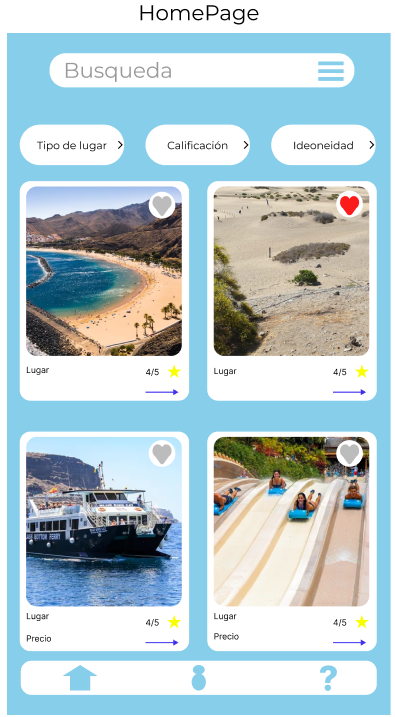
\includegraphics[width=\linewidth]{figures/homepage.png}
		\caption{Design for the home page of our app}
		\label{fig:homepage}
	\end{subfigure}
	\hfill
	\begin{subfigure}[T]{0.4\linewidth}
		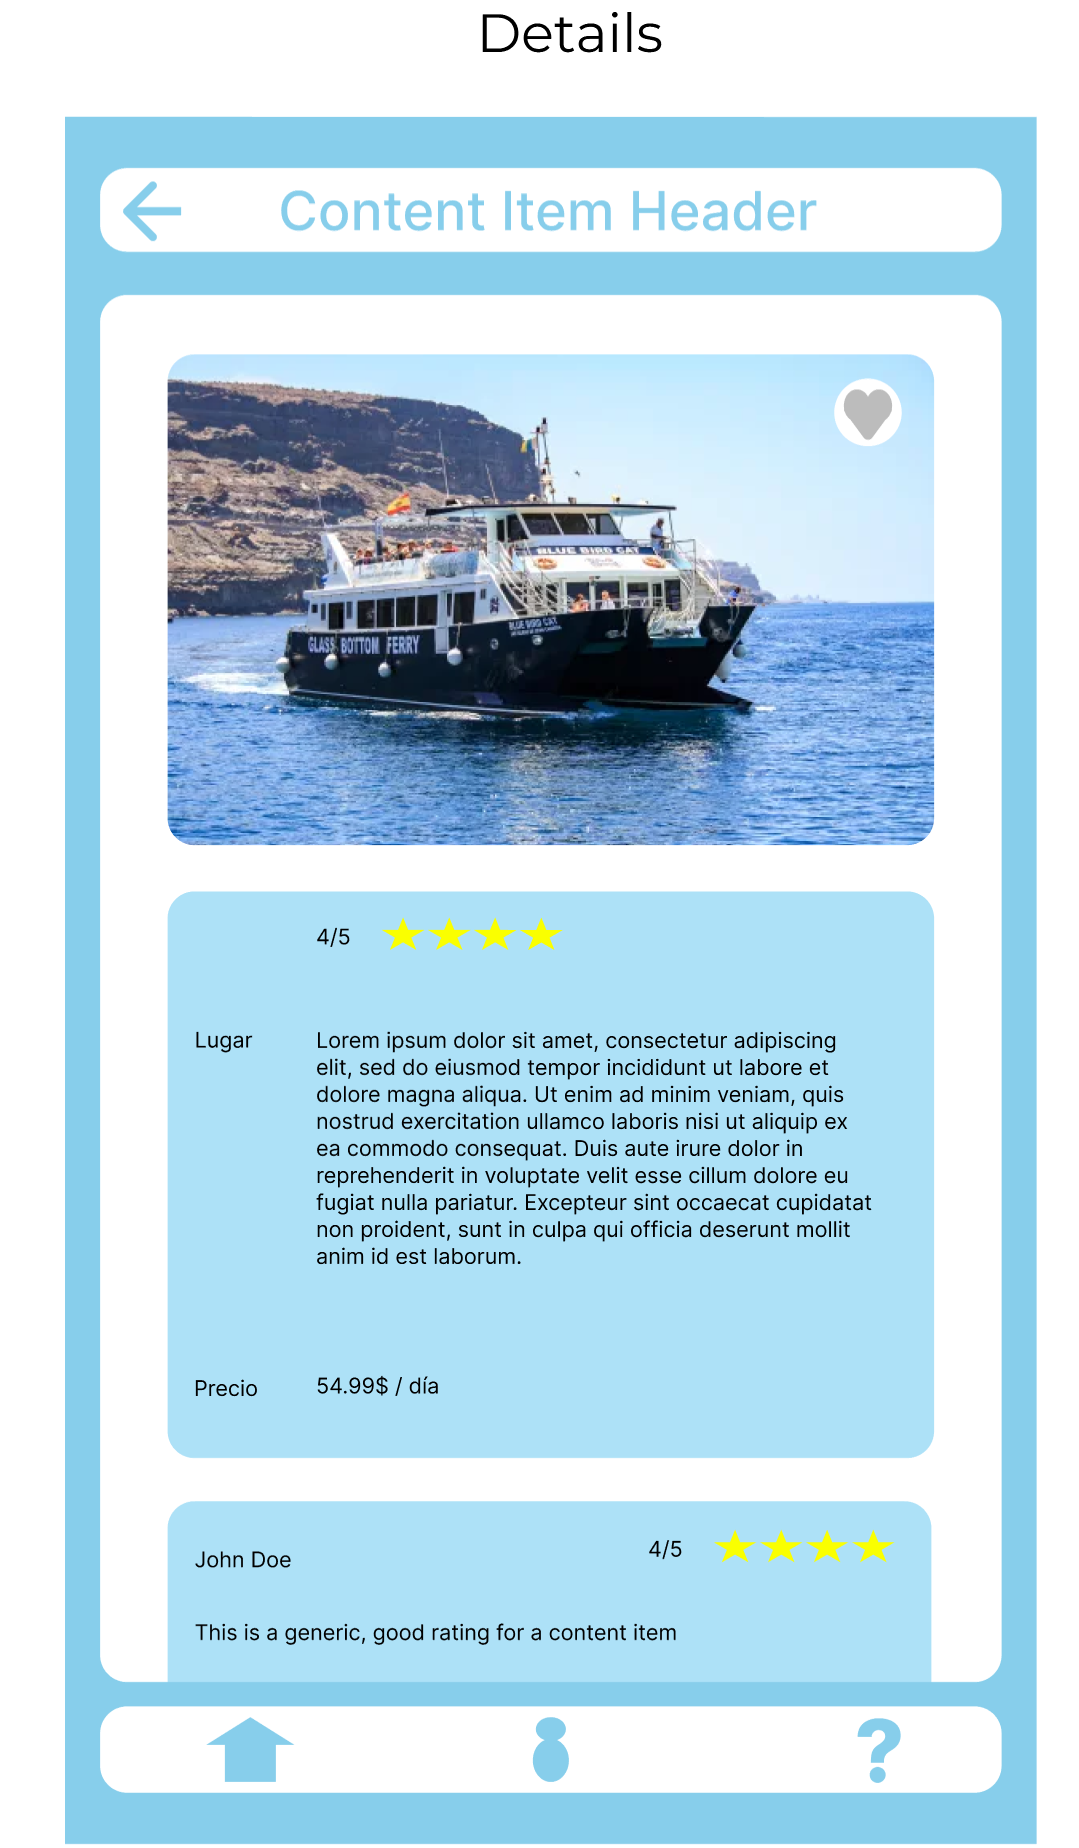
\includegraphics[width=\linewidth]{figures/details.png}
		\caption{Design for the content item details page of our app}
		\label{fig:details}
	\end{subfigure}
\end{figure}

\begin{figure}
	\centering
	\begin{subfigure}[T]{0.4\linewidth}
		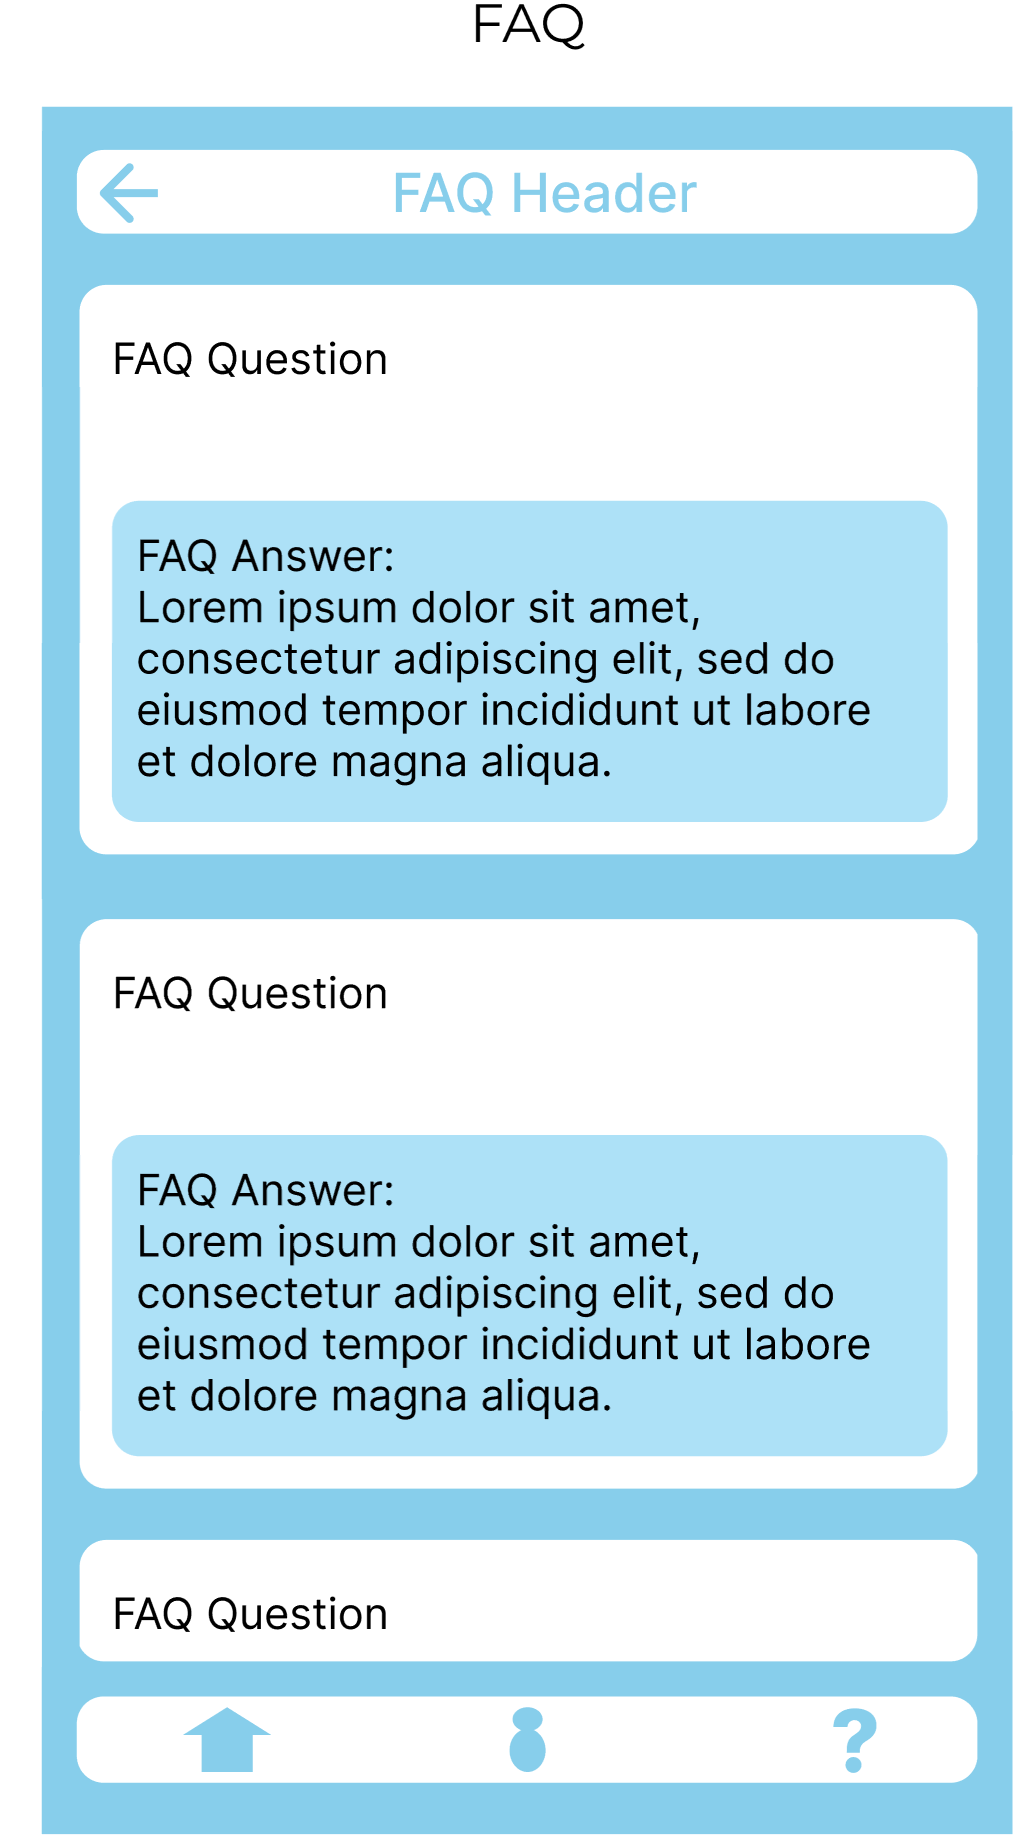
\includegraphics[width=\linewidth]{figures/FAQ.png}
		\caption{Design for the FAQ page of our app}
		\label{fig:FAQ}
	\end{subfigure}
	\hfill
	\begin{subfigure}[T]{0.4\linewidth}
		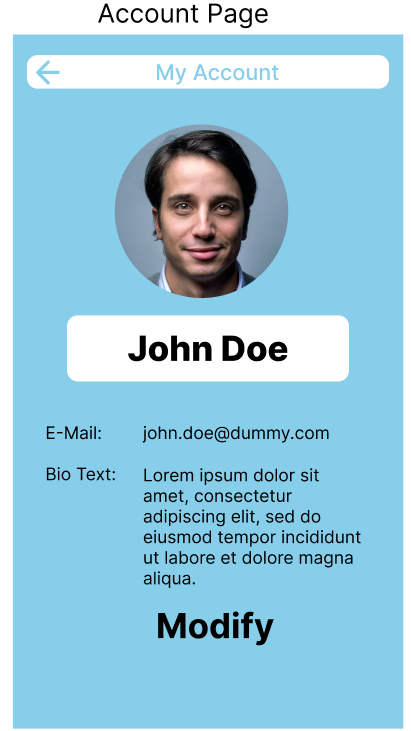
\includegraphics[width=\linewidth]{figures/account.png}
		\caption{Design for the account page of our app}
		\label{fig:account}
	\end{subfigure}
\end{figure}

\begin{figure}
	\centering
	\begin{subfigure}[T]{0.4\linewidth}
		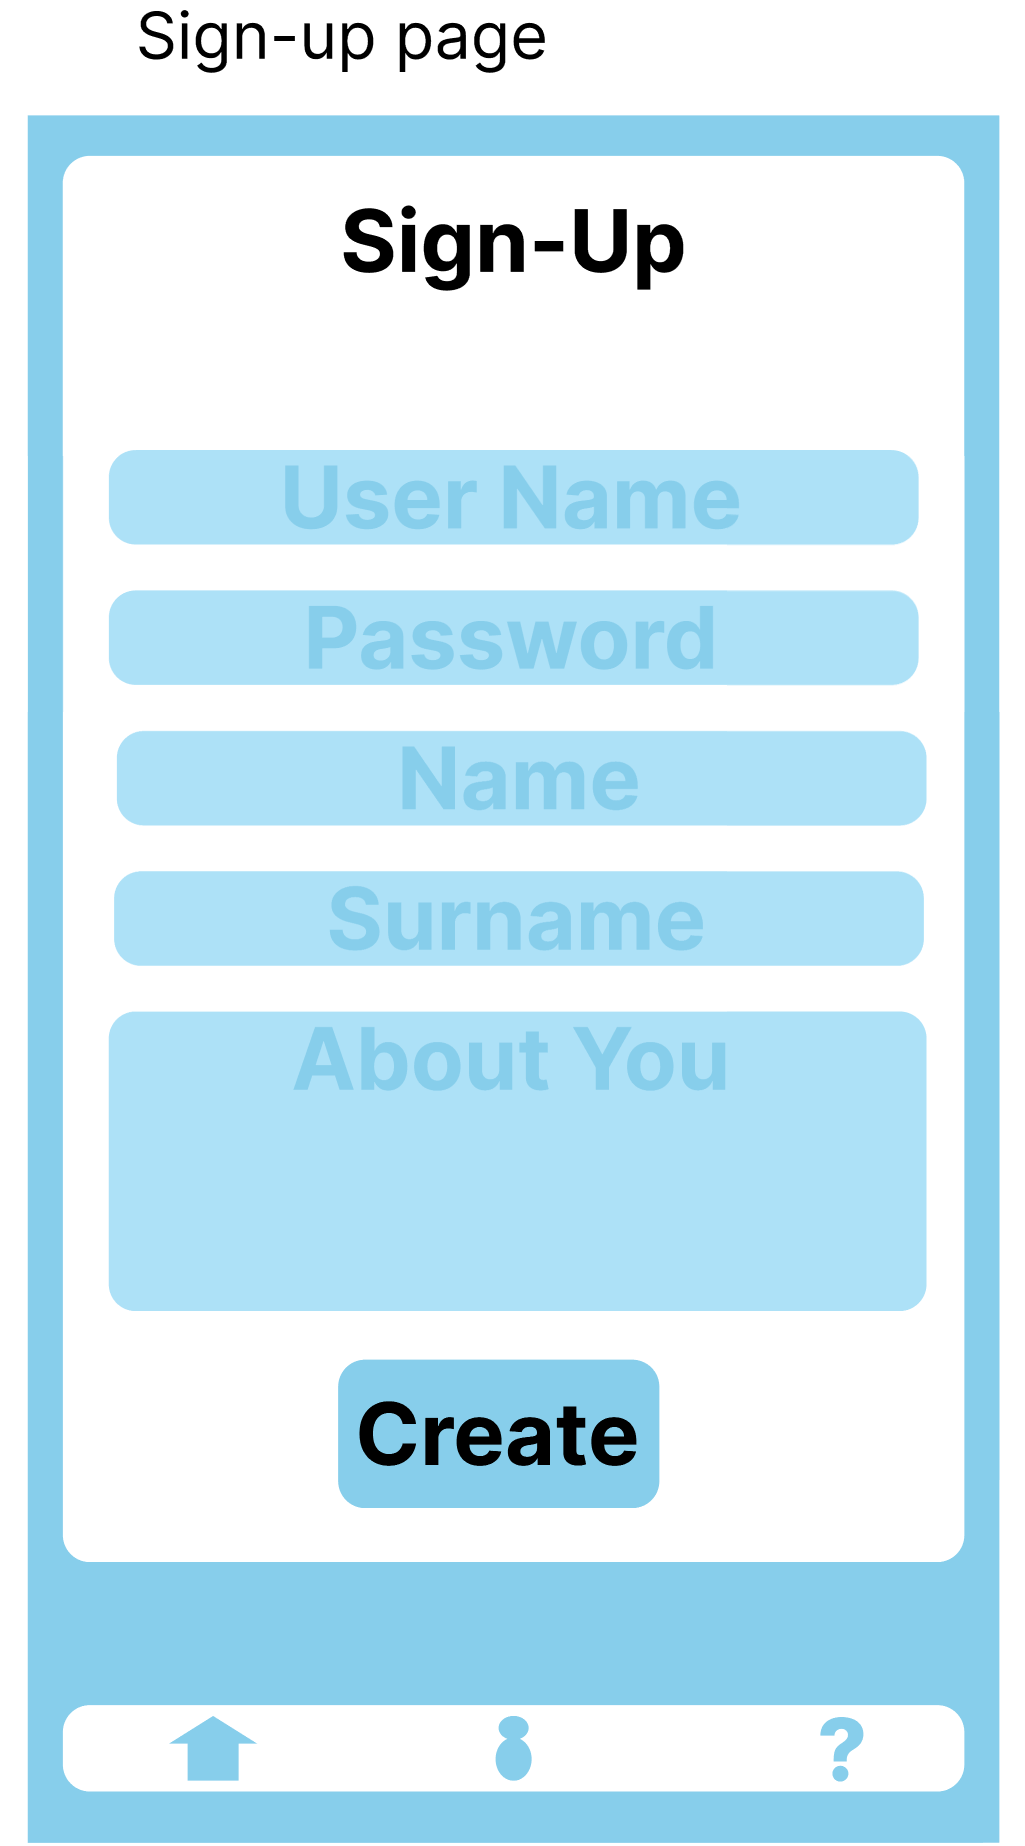
\includegraphics[width=\linewidth]{figures/sign_up.png}
		\caption{Design for the sign-up page of our app}
		\label{fig:sign_in}
	\end{subfigure}
	\hfill
	\begin{subfigure}[T]{0.4\linewidth}
		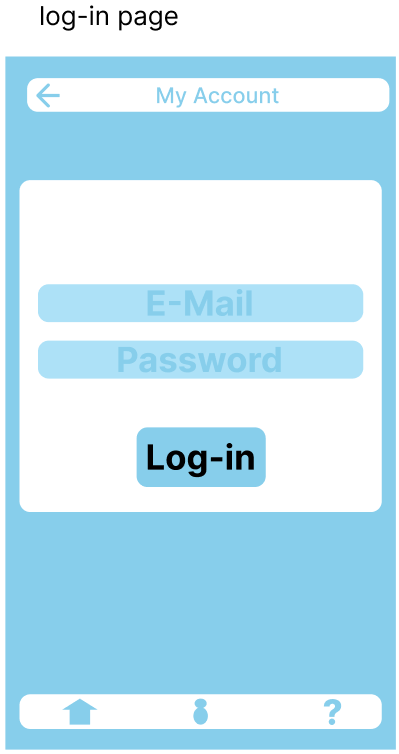
\includegraphics[width=\linewidth]{figures/log_in.png}
		\caption{Design for the log-in page of our app}
		\label{fig:log_in}
	\end{subfigure}
\end{figure}
